\documentclass[a5paper,12pt]{article}
\usepackage{../../style}


\newcommand{\montitre}{Algo }


\begin{document}

\fiche{Introduction}
\titre{Principes de la POO} : 
\begin{enumerate}
	\item Objet
	\item Méthode
	\item Classe
	\item Hiérarchie de classes
\end{enumerate}

\titre{Exemple : définition de la structure conditionnelle en smallTalk}\\
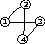
\includegraphics[width=180px]{Images/fig1.pdf}

\titre{Plan de cours}
\begin{enumerate}
	\item Introduction
	\item Concepts de base (objet, classe, envoi de message, hiérarchie)
	\item Illustrations et exemples (Java, Simula, SmallTalk
	\item Etude comparative de LO
	\item TP (Java, Eclipse)
\end{enumerate}

\titre{Histoire d'Ada}
Le département de la défense américain (Dod) est : 
\begin{itemize}
	\item Plus gros consommateur de logiciels
	\item 1968 - 73 : Le coût des SI augmente et le coût du matériel chute
	\item 73 : 7,5 milliards de dollars pour les Si
	\item 75 : 450 langages différents
	\item Réutilisabilité et partage de code inexistants
	\item 1983 : naissance d'Ada en réponse à la crise du logiciel et pour résoudre les pbs liés au dev de gros logiciels
	\item non issu d'un projet académique ou de recherche interne
\end{itemize}
Idée : Un seul langage incorporant tous les bons concepts de GL.\\

\titre{Paradigmes de programmation}
\begin{itemize}
	\item impérative
	\item fonctionnelle
	\item logique
	\item objet
	\item par contraintes
\end{itemize}

\newpage

\titre{Les domaines révolutionnés par la POO}
\begin{itemize}
	\item Génie logiciel (analyse, conception, programmation)
	\item Bases de données
	\item Intelligence artificielle (représentation des connaissances, programmation par agents)
\end{itemize}

\titre{Quel objet ?}
\begin{itemize}
	\item Des problématiques différentes $\rightarrow$ Des approches objet différentes
	\item Une préoccupation commune (approche modulaire de la complexité)
\end{itemize}
Pour distinguer les approches différentes, on change le voc :
\begin{itemize}
	\item Génie Logiciel : Objet
	\item IA : Schéma
	\item Ingénierie collaborative : Agent
	\item Bases de données : RDF
\end{itemize}

\titre{Quels languages :}
\begin{itemize}
	\item Java sous éclipse principalement
	\item Simula
	\item SmallTalk
\end{itemize}


\fiche{Connexité}
\titre{Chemin :} Un chemin dans un graphe $G=(S,A)$ est une séquence de sommets $C = [ c_1,\ldots,c_n ]$ telle que $(c_i,c_{i+1}) \in A \forall i \in \{ 1 .. n-1 \}$ \\
 
\titre{Longueur :} La longueur de $C$ est $n-1$ \\

\titre{Chemin simple :} $i\neq j \impl c_i \neq c_j$ \\

\titre{Cycle :} Un cycle est un chemin "simple" mais avec $c_1 = c_n$, sauf les chemins du type $[u,v,u]$ des graphes non orientés. \\

\titre{Critère d'isomorphie :} Deux graphes isomorphes ont le même nombre de cycles de chaque longueur. Ce critère est nécessaire mais non suffisant. (fig6)\\

\titre{Condition nécessaire :} \\
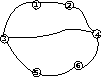
\includegraphics[width=100px]{Images/fig4.pdf} \hspace{1cm} 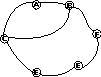
\includegraphics[width=100px]{Images/fig5.pdf} \\

\titre{Condition non suffisante :} \\

\includegraphics[width=100px]{Images/fig6.pdf} \\

\titre{Composante connexe :} Soit $G=(S,A)$ un graphe non orienté. Une commposante connexe de $G$ est un sous ensemble maximal de sommets $S'$ tel que pour toute paire de sommets $(u,v)$ de $S'$, il existe un chemin de $u$ à $v$. \\

\titre{Connexité :} Un graphe est dit connexe s'il ne contient qu'une seule composante connexe. \\

\titre{Composante fortement connexe :} Soit $G=(S,A)$ un graphe orienté. Une commposante fortement connexe de $G$ est un sous ensemble maximal de sommets $S'$ tel que pour toute paire de sommets $(u,v)$ de $S'$, il existe un chemin de $u$ à $v$. \\

\titre{Graphe fortement connexe :} Ses sommets forment une composante fortement connexe. \\



\fiche{Arbres}
\titre{Arbre :} Une arbre est un graphe non orienté connexe et sans cycle. \\

\titre{Forêt :} Un graphe est une forêt si chacune de ses composantes connexes est un arbre. \\

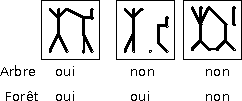
\includegraphics[width=300px]{Images/fig7.pdf} \\

\titre{Arbre couvrant :} A partir d'un graphe connexe, on peut se réduire à un arbre en "coupant" des arêtes. C'est l'arbre couvrant.

\titre{Simplification :} On suppose que les sommets sont $\{1, \ldots , n\}$ \\

\titre{Matrice d'adjacence :} \\$M = \displaystyle{(m_{ij})_{1\leq i \leq n,1\leq j \leq n}}$ où $m_{ij} = \left\{ \begin{array}{l} 1 \mathrm{si} (i,j) \in A \\ 0 \mathrm{sinon} \end{array} \right.$

\titre{Exemple : }\\
\begin{minipage}{0.4\linewidth}
$\left[\begin{array}{ccccc}
	0 & 1 & 0 & 0 & 1 \\
	0 & 0 & 0 & 1 & 0 \\
	0 & 1 & 0 & 1 & 0 \\
	0 & 0 & 0 & 0 & 0 \\
	0 & 1 & 0 & 1 & 1 \\
\end{array}\right]$
\end{minipage}
\begin{minipage}{0.4\linewidth}
\hspace{2cm} 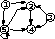
\includegraphics[width=100px]{Images/fig8.pdf}
\end{minipage}

On utilisera donc un tableau bidimensionnel. \\

\titre{Graphes par listes d'adjacences :} A chaque sommet est associée une liste qui contient les sommets qui lui sont adjacents. \\

On utilisera donc un tableau de listes.  \\

\titre{Exemple :}\\
$\begin{array}{l}
	1 : 5,2 \\
	2 : 4 \\
	3 : 2,4 \\
	4 : \\
	5 : 2,4,5 \\
\end{array}$ \newpage

\titre{Comparaison des deux représentations :} \\
\begin{tabular}{l|p{4cm}|p{4cm}}
	& Matrice & Listes \\ \hline
Espace & $O(n^2)$ & $O(n^2)$ au pire cas, $O(n)$ au meilleur cas \\ \hline
Initialisation & Pour i de 1 à n faire (Pour j de 1 à n faire) M[i,j]=0, donc $O(n^2)$ & Pour i de 1 à n faire (T[i] = liste vide), donc $O(n)$ \\ \hline
Test d'adjacence & $O(1)$ & $O(n)$ au pire cas, $O(\mathrm{nbVois})$ au cas moyen, $O(1)$ au meilleur cas \\ \hline
Afficher les voisins & $O(n)$ & $O(n)$ au pire cas, $O(\mathrm{nbVois})$ au cas moyen, $O(1)$ au meilleur cas \\ \hline
Ajouter l'arête $(u,v)$ & T[$u$].insererEnTete($v$) $O(1)$ & M[u,v] = 1 $O(1)$ \\ \hline
\end{tabular} \\

\titre{Conclusion :} 
\begin{itemize}
	\item Si on a un grand graphe avec peu d'arêtes par rapport au nombre de sommets (ou alors vraiment beaucoup, dans ce cas on peut inverser), la représentation en listes est préférable.
	\item Si on a un petit graphe, une matrice est plus simple à manipuler et pas plus couteuse
	\item Pour les autres cas, le choix dépendra du contexte.
\end{itemize}


\fiche{Parcours de graphes}
\titre{Principe :} A partir d'un sommet, on calcule un arbre couvrant sur les sommets accessibles à partir de ce sommet. \\
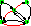
\includegraphics[width=200px]{Images/fig9.pdf}\\

\titre{Parcours en largeur :} On regarde les voisins du sommet, puis leurs voisins et ainsi de suite. Cela produit des chemins de longueur minimales du sommet de départ à tous les autres. \\

\titre{Exemple :} \\

\includegraphics[width=200px]{Images/fig10.pdf}\\
\begin{tabular}{l|l|l|l|l|l|l|l|l}
 vu & V & V & V & V & V & V & V & V
\end{tabular} \\

\begin{tabular}{l|l|l|l|l|l|l|l|l}
 pere & 2 & - & 6 & 3 & 1 & 2 & 6 & 7
\end{tabular} \\

\begin{tabular}{l|l|l|l|l|l|l|l|l}
 dist & 1 & 0 & 2 & 3 & 2 & 1 & 2 & 3
\end{tabular} \\

F : $\bar{2}$ $\bar{1}$ $\bar{6}$ $\bar{5}$ $\bar{3}$ $\bar{7}$ $\bar{4}$ $\bar{8}$ \\
u = 2 
v = 1 
v = 6 \\
u = 1 
v = 2 (déjà vu) 
v = 5 \\
u = 6 
v = 2 (déjà vu) 
v = 3 
v = 7 \\
u = 5 
v = 1 (déjà vu) \\
u = 3 
v = 4 
v = 6 (déjà vu) 
v = 7 (déjà vu) 
u = 7 
v = 3 (déjà vu) 
v = 6 (déjà vu) 
v = 8 \\
u = 4 (tous voisins déjà vus) \\
u = 8 (tous voisins déjà vus) \\

\titre{Complexité en temps :} On simplifie en supposant que le graphe a $n$ sommets et $m$ arretes\\
\begin{tabular}{l|p{4cm}|p{4cm}}
lignes & Listes & Matrices \\ \hline
1 à 4 & $O(1)$ & $O(1)$ \\ \hline
5 à 8 & $O(n)$ & $O(n)$ \\ \hline
9 à 11 & $O(1)$ & $O(1)$ \\ \hline
15 à 19 & $O(1)$ & $O(1)$ \\ \hline
14 & $O(nbVois)$ ou au pire $O(n)$ & $O(n)$ \\ \hline
14 à 19 & $O(nbVois)$ & $O(n)$ \\ \hline
12 & $n$ itérations & $n$ itérations \\ \hline
12 à 19 & $O(m)$ & $O(n^2)$ \\ \hline
\end{tabular}

\newpage

\titre{Parcours en profondeur :} On part dans une direction et tant qu'on peut on avance. Quand on est coincé on recule d'un cran et on voit si il y a une autre direction. \\

\titre{Exemple :} \\

\includegraphics[width=200px]{Images/fig11.pdf} \\

\begin{tabular}{l|l|l|l|l|l|l|l|l}
 vu & V & V & V & V & V & V & V & V
\end{tabular} \\

\begin{tabular}{l|l|l|l|l|l|l|l|l}
 pere & - & 1 & 2 & 3 & 2 & 8 & 8 & 2
\end{tabular} \\

\begin{tabular}{l|l|l|l|l|l|l|l|l}
 d & 1 & 2 & 3 & 4 & 7 & 10 & 12 & 9
\end{tabular} \\

\begin{tabular}{l|l|l|l|l|l|l|l|l}
 f & 16 & 15 & 6 & 5 & 8 & 11 & 13 & 14
\end{tabular} \\

Pile des appels récursifs : \\
u = 7 $\rightarrow$ 6(vu), 8(vu) FINI \\
u = 6 $\rightarrow$ 1(vu), 5(vu) FINI \\
u = 8 $\rightarrow$ $\bar{6}$,$\bar{7}$ FINI \\
u = 5 $\rightarrow$ 1(vu), 4(vu) FINI \\
u = 4 $\rightarrow$ 2(vu) FINI \\
u = 3 $\rightarrow$ $\bar{4}$ FINI \\
u = 2 $\rightarrow$ $\bar{3}$,$\bar{5}$,$\bar{8}$ FINI \\
u = 1 $\rightarrow$ $\bar{2}$,5(vu),8(vu) FINI \\
temps : 16 \\

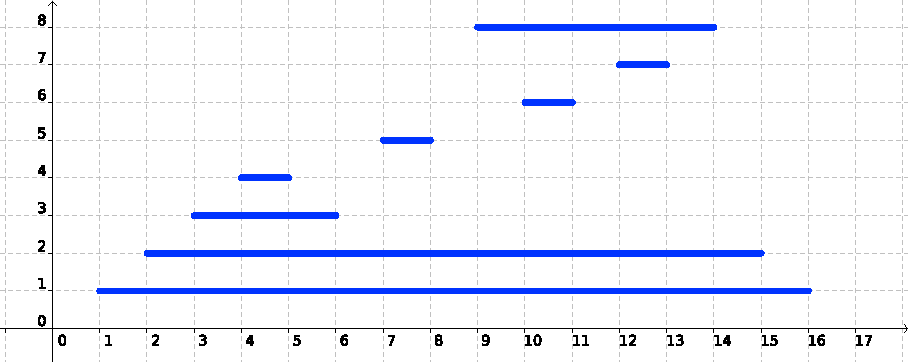
\includegraphics[width=300px]{Images/fig12.pdf} \\


\fiche{TD 1}
\titre{Question 1}\\
\\
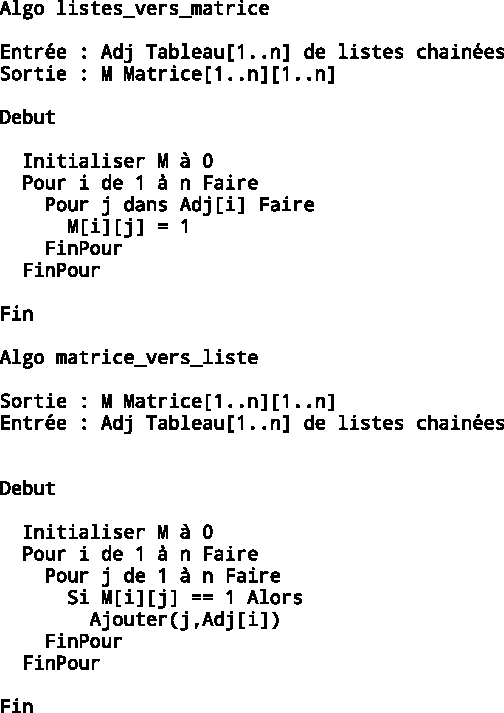
\includegraphics{Images/fig19.pdf}
\\
\newpage
\titre{Question 2}\\
\\
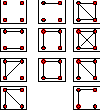
\includegraphics[width=200px]{Images/fig20.pdf}
\\
\\
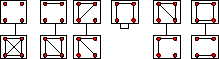
\includegraphics[width=300px]{Images/fig21.pdf}
\\
\titre{Question 3}
\begin{enumerate}
	\item $K_n$ possède $\frac{n(n-1)}{2}$ arêtes.
	\item $\bar{K_n}$ possède 0 arête
	\item $O(n^2)$
\end{enumerate}

\titre{Question 4} Il y a deux sous graphes isomorphes à $K_3$ et aucun isomorphe à $\bar{K_3}$
\newpage
\titre{Question 5} \\
\\

\includegraphics[width=100px]{Images/fig23.pdf}
\\
\titre{Question 6} 
\begin{enumerate}
	\item .\\ 
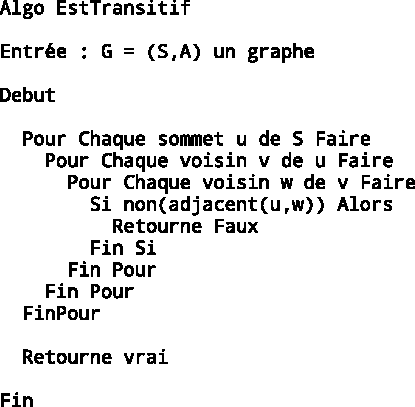
\includegraphics{Images/fig24.pdf}
	\item $O(n^2)$
	\item .\\
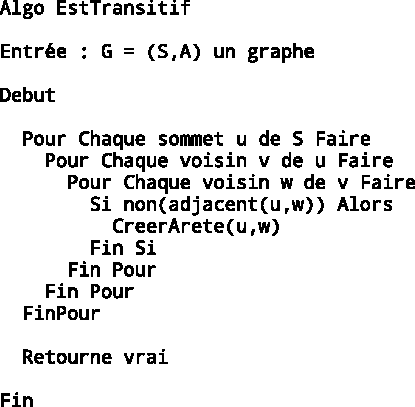
\includegraphics{Images/fig25.pdf}
	\item $O(n^2)$
	\item Faire mieux ???
\end{enumerate}

\titre{Question 7} Il faut commencer par enlever une allumette \\
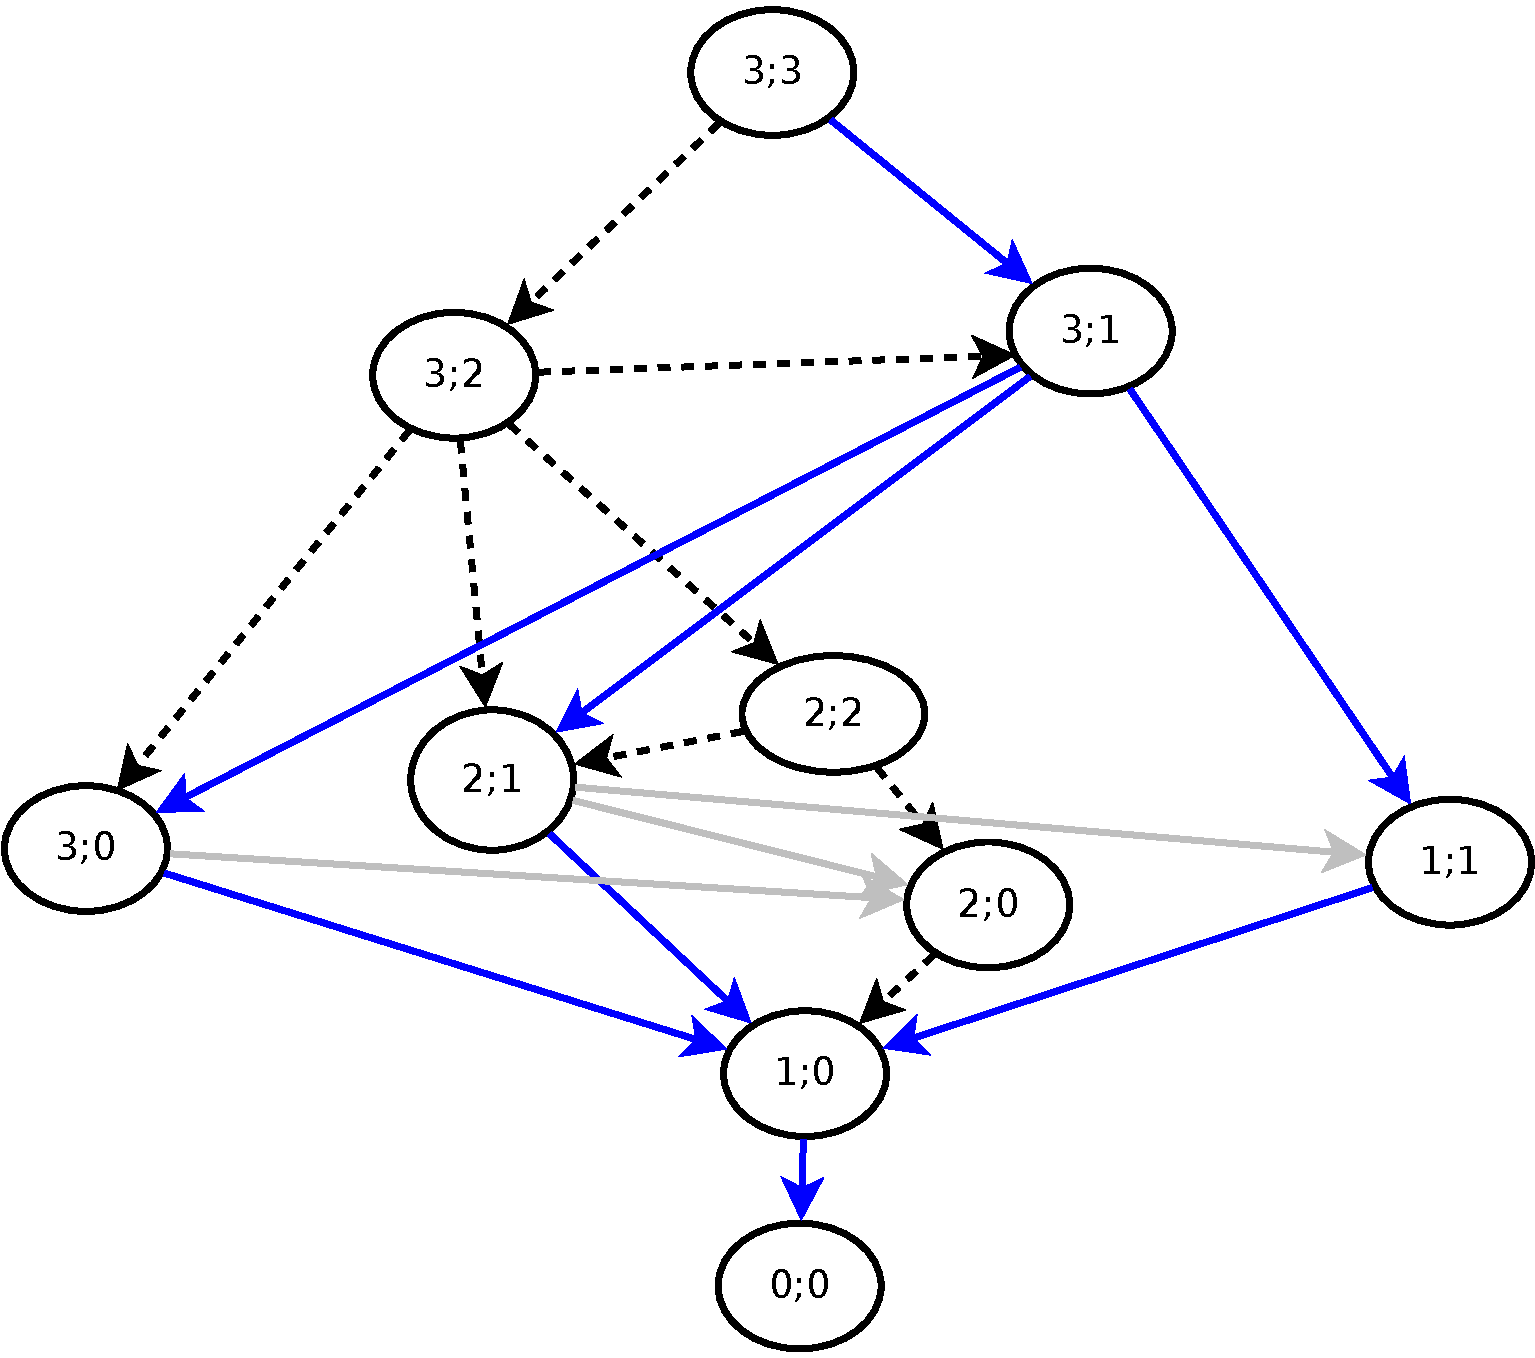
\includegraphics[width=250px]{Images/fig26.pdf} \\

\titre{Question 8} P = passeur, C = choux, B = chèvre (bêêê), L = loup \\
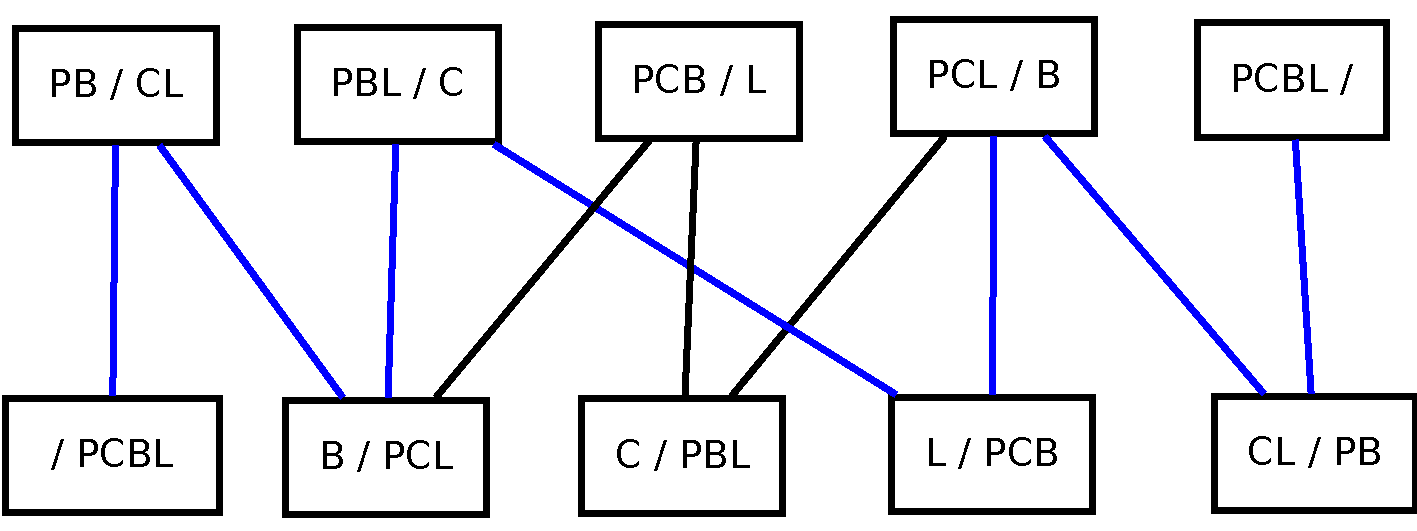
\includegraphics[width=250px]{Images/fig27.pdf} \\

\titre{Question 9} \\
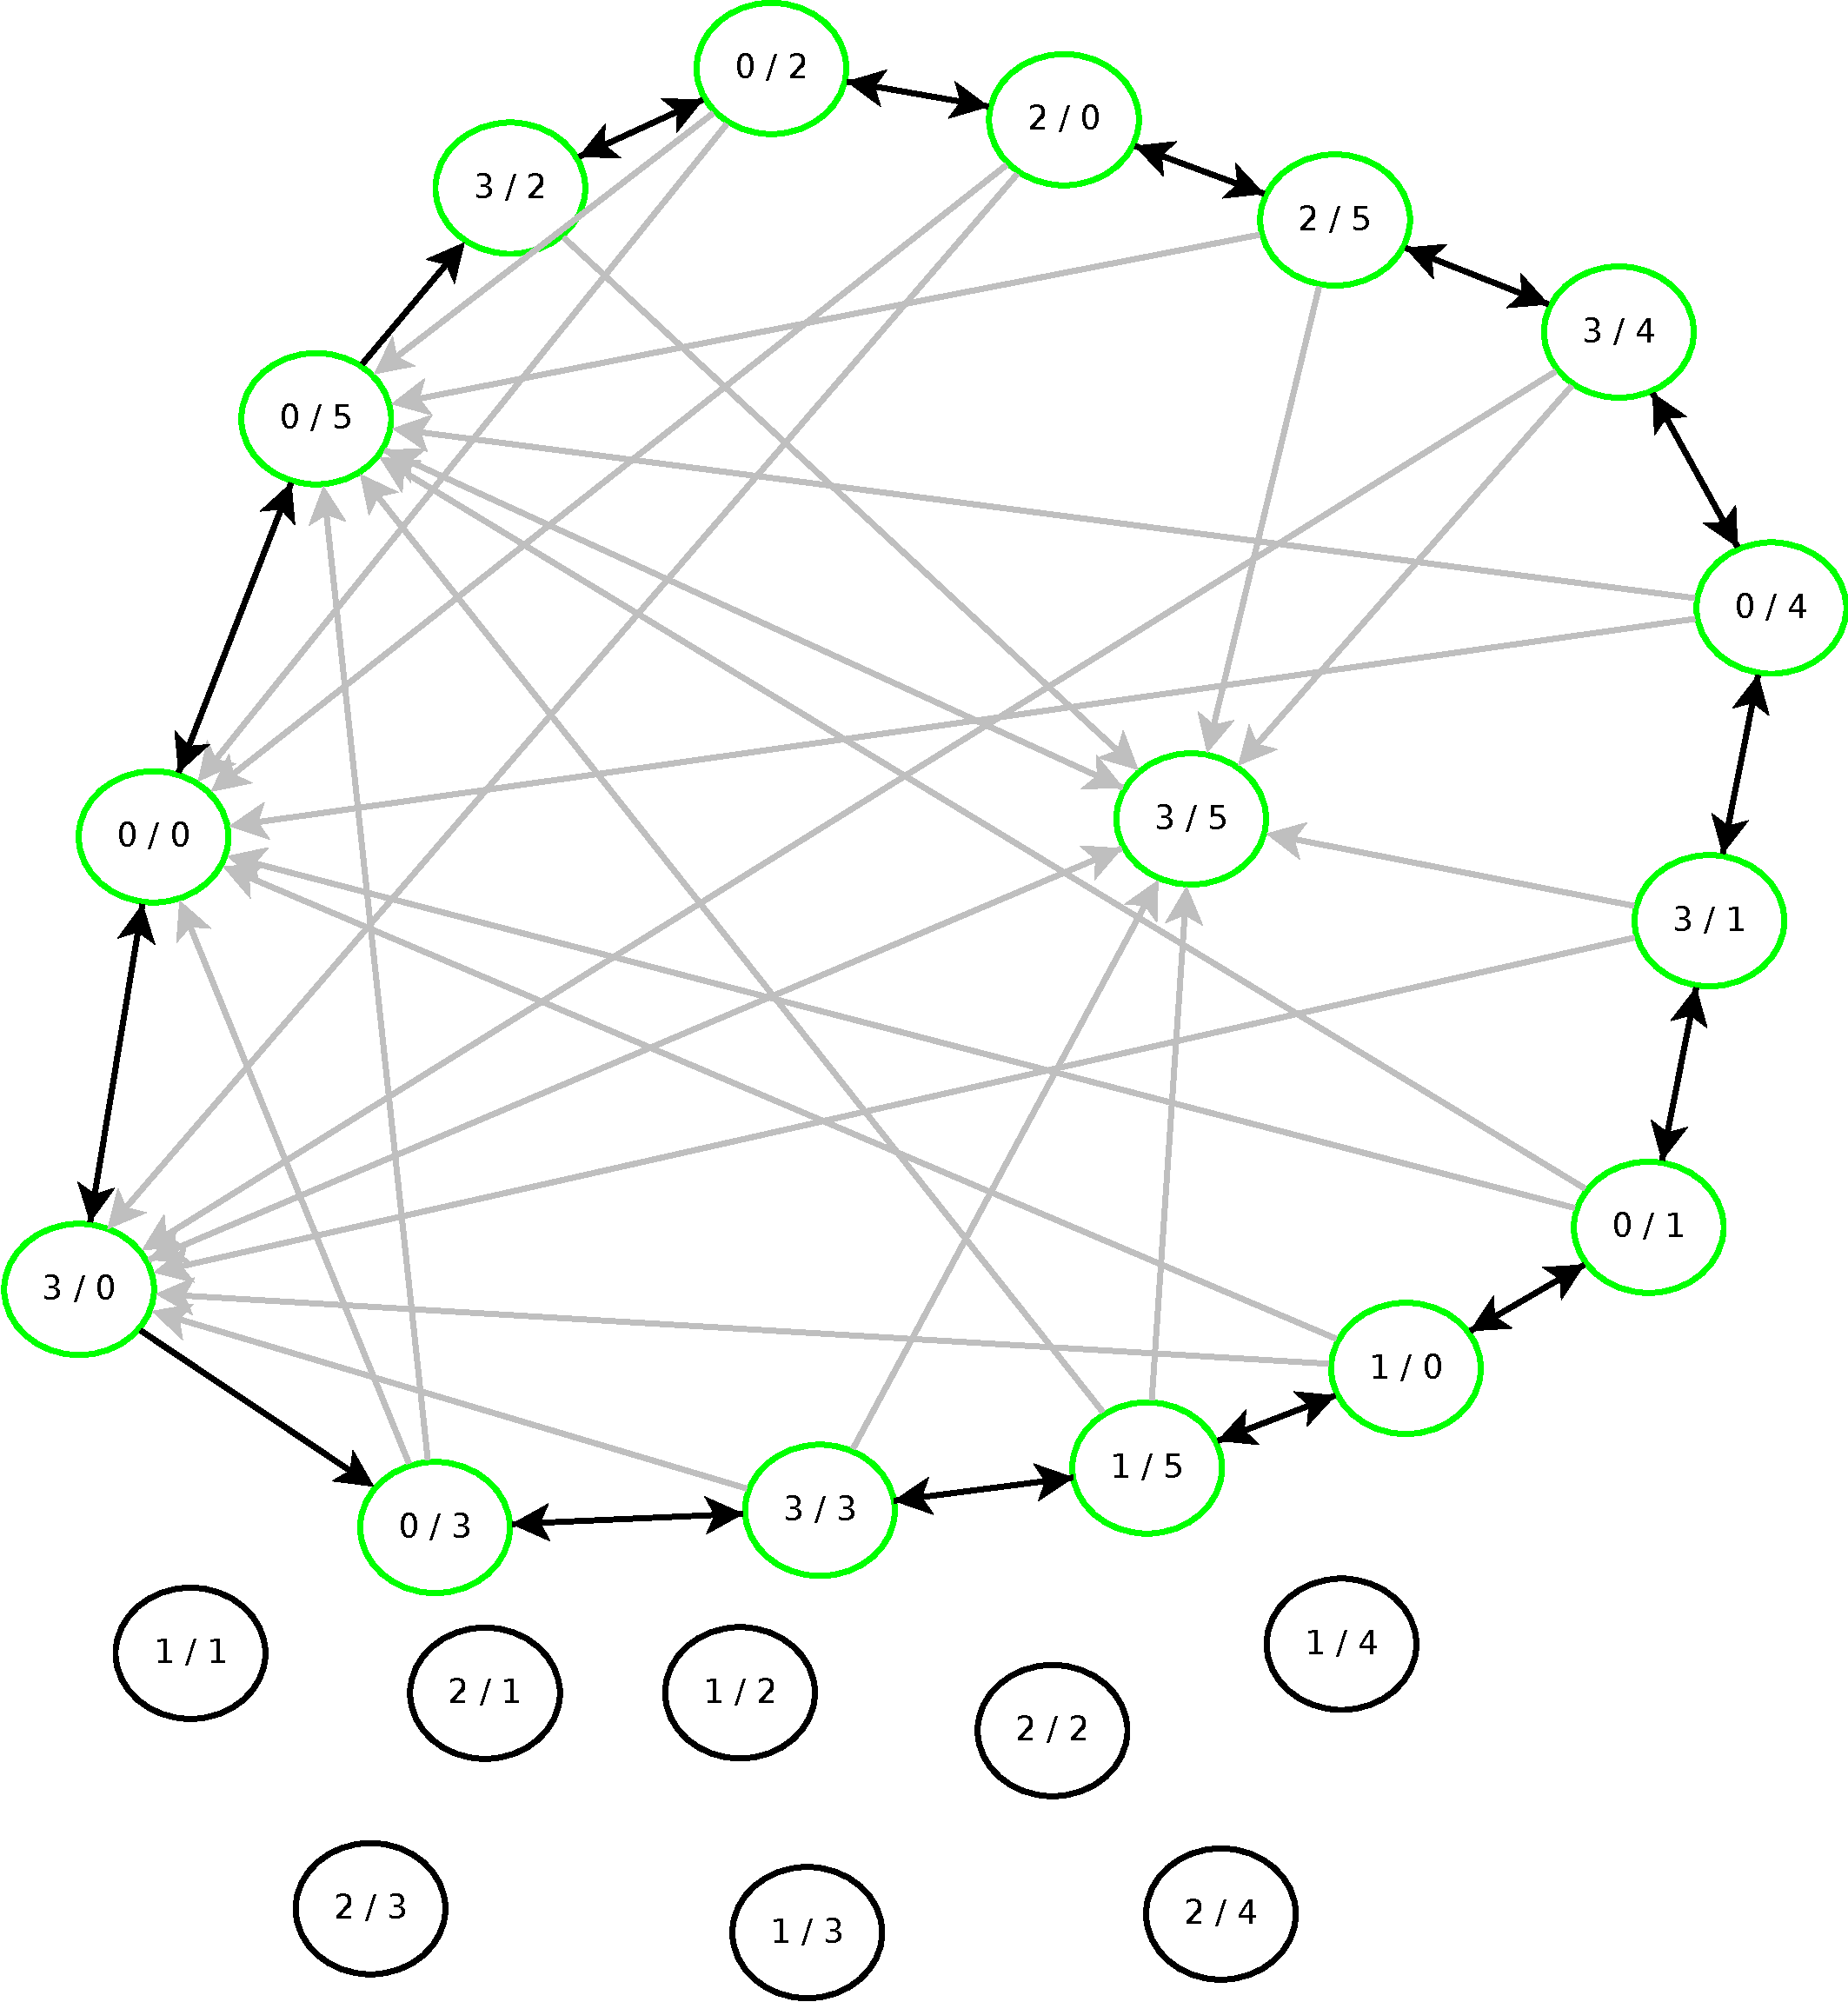
\includegraphics[width=300px]{Images/fig28.pdf} \\


\fiche{TD 2}
\titre{Question 1 b}
\begin{enumerate}
	\item Oui (voir contre exemple)
	\item Oui (voir contre exemple)
	\item Non pour un graphe connexe (le nombre d'arêtes d'un arbre dépend uniquement du nombre de noeud car chaque fois qu'on ajoute un noeud dans un arbre on ajoute une arête (sauf la racine))
\end{enumerate}

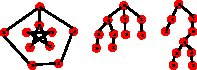
\includegraphics[width=300px]{Images/fig13.pdf}

\titre{Question 2}
\begin{enumerate}
	\item .\\ 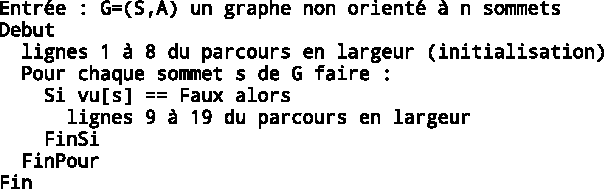
\includegraphics{Images/fig14.pdf}
	\item La forêt couvrante d'un graphe connexe est un arbre
\end{enumerate}

\titre{Question 3} Il suffit de rajouter un compteur dans l'algorithme précédent :\\
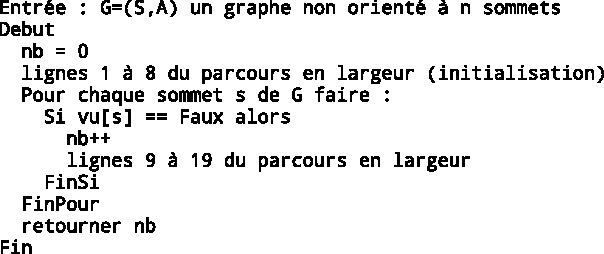
\includegraphics{Images/fig15.pdf}

\titre{Question 4} 
\begin{enumerate}
	\item .\\ 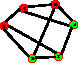
\includegraphics[width=100px]{Images/fig16.pdf}
	\item Un simple triangle n'est pas biparti
	\item On part du parcours en largeur ou en profondeur : on donne une couleur au premier voisin, puis l'autre à tous ces voisins qui n'ont pas de couleur, pour les autres voisins on regarde si ils sont de couleur différente, sinon on s'arrête en répondant non. \\ 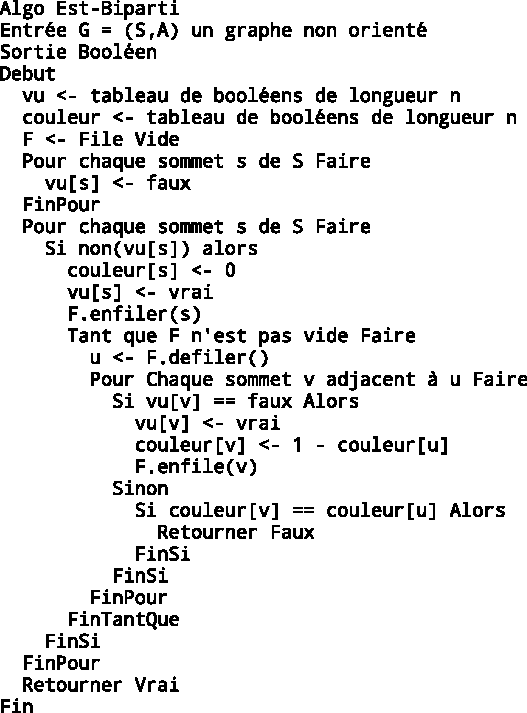
\includegraphics{Images/fig17.pdf}
\end{enumerate}

\titre{Question 5} \\ 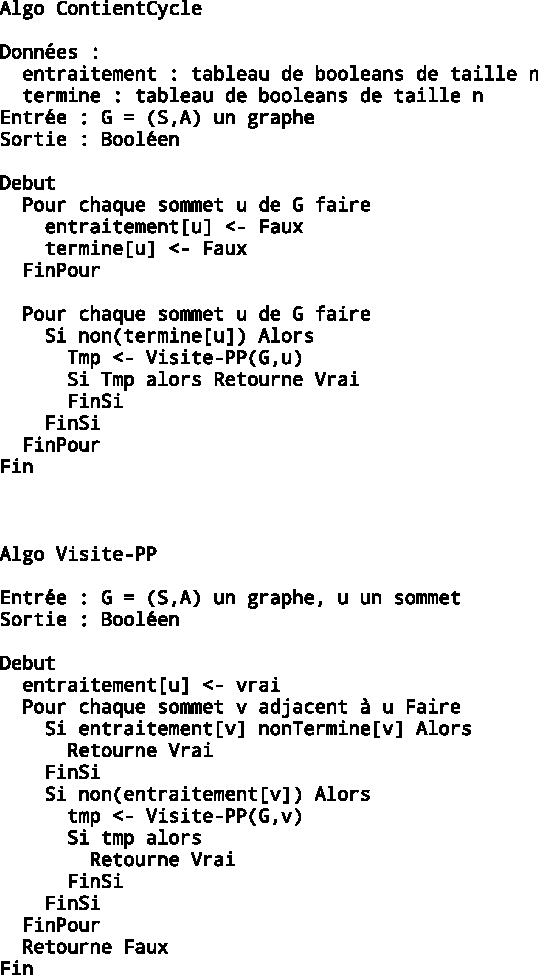
\includegraphics{Images/fig18.pdf}



\fiche{Chemins de longueur minimale}
\titre{Calcul des CLM : Chemins de Longueur Minimale}
\begin{enumerate}
	\item D'un sommet à un autre (on fait le 2 et on extrait le bon chemin)
	\item D'un sommet à tous les autres (Dijkstra)
	\item De tous les sommets à un autre (On inverse les arêtes du graphe et on fait 2)
	\item De tous les sommets vers tous les sommets (Floyd-Warshall)
\end{enumerate}

\titre{Définition :} Soit $G=(S,A)$ un graphe et $p$ sa fonction de pondération. Un \titre{Chemin de Longueur Minimale} du sommet $u$ au sommet $v$ est un chemin de $[s_0,\ldots,s_k]$ avec $s_0=u$, $s_k=v$ et $\sum p(s_i,s_{i+1})$ minimal.\\

\titre{Arbre de CLM :} Un arbre couvrant enraciné en un sommet $s$ tel que l'unique chemin de $s$ à un sommet $u$ de cet arbre est un CLM du graphe de départ. \\

\titre{Remarques :} 
\begin{itemize} 
	\item L'arbre de CLM existe.
	\item Soit $[s_0,\ldots,s_k]$ un CLM de $s_0$ à $s_k$. Alors pour tout $i\in\{1,\ldots,k-1\}$ on a $[s_0,\ldots s_i]$ est un CLM de $s_0$ à $s_i$
\end{itemize}

\titre{Algorithme de Dijkstra :} Meme principe que l'algo de Prim à la différence que cle[u] est la longueur du plus court chemin connu du sommet de départ au sommet u.\\

\titre{Algorithme de Floyd-Warshall :} L'idée est de construire dynamiquement une suite de matrices $M_0,\ldots,M_n$ telles que $m_{k_{i,j}}$ est le cout du plus court chemine de $i$ à $j$ en utilisant comme sommets intermédiaires les sommets $1,2,\ldots ,k$


\fiche{Problèmes de maximisation}
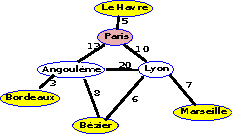
\includegraphics[width=200px]{Images/fig29.pdf}
\titre{Problème du Flot Maximal :} Voici un réseau de transport : \\
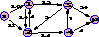
\includegraphics[width=200px]{Images/fig30.pdf}\\
\begin{enumerate}
	\item Un graphe orienté dont les arêtes sont pondérées positivement par une fonction de capacité
	\item Une source à production illimitée
	\item Un puit p à consommation illimitée
\end{enumerate}

\titre{Exemple :}
\begin{enumerate}
	\item boite 1 : $[s,2,4,p]$
	\item boite 2 : $[s,2,1,3,p]$
\end{enumerate}
Une contrainte : Aucune accumulation : ce qui entre est égal à ce qui sort\\
On trouve ici un flot maximal de 23 : \\
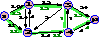
\includegraphics[width=200px]{Images/fig31.pdf}\\

\titre{Méthode pour trouver le flot maximal :} Un flot sur $G$ est une fonction $f$ qui a chaque arc $(u,v)$ associe une quantité $f(u,v)$  telle que :
\begin{enumerate}
	\item $f$ respecte les capacités : $f(u,v) \leq c(u,v)$
	\item Symétrie : $f(u,v) = -f(v,u)$
	\item Conservation du flot : Pour chaque sommet $u$ de $G$ autre que $s$ et $p$ on a $\displaystyle{\sum_{v\in S} = 0}$ (manière formelle de dire : ce qui entre est égal à ce qui sort).
	\item \titre{Flot du réseau :} $F = \displaystyle{\sum_{v\in S} f(s,v)} = \displaystyle{\sum_{v\in S} f(v,p)}$
\end{enumerate}

\titre{Problème du Flot maximal :} Etant donné un réseau de transport $G$, trouver un flot $f$ qui maximise le flot du réseau. \\ 

\titre{Remarque :} Si il y a $m$ sources et $n$ puits, il ne peut y avoir aucune arête qui entre dans une source ou sort d'un puit :\\
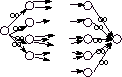
\includegraphics[width=200px]{Images/fig32.pdf}\\

\titre{Annulation des flots}\\
Principe général : \\
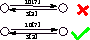
\includegraphics[width=100px]{Images/fig33.pdf}\\
Ajout d'un flux dans le cas de double arête : \\
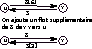
\includegraphics[width=100px]{Images/fig34.pdf}\\
Ajout d'un flux dans le cas d'une simple arête :\\
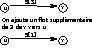
\includegraphics[width=100px]{Images/fig35.pdf}\\

\titre{Réseau résiduel :} Etant donné un réseau de transport $G=(S,A)$, sa fonction de capacité $c$ et un flot $f$ sur $G$. Le réseau résiduel est le même graphe muni de la fonction de capacité $c_f = c(u,v) - f(u,v)$\\

\titre{Exemple :}\\
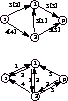
\includegraphics[width=100px]{Images/fig36.pdf}\\

\titre{Remarque :} Soit $f'$ un flot valide sur le graphe résiduel, alors $f+f'$ est un flot valide sur $G$.\\
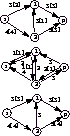
\includegraphics[width=100px]{Images/fig37.pdf}\\
On trace encore le résiduel avec ce nouveau flot : \\
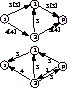
\includegraphics[width=100px]{Images/fig38.pdf}\\

\titre{Propriété :} S'il n'existe aucun chemin de $s$ à $p$ dans le graphe résiduel, alors $f$ est maximal. \\

\titre{Algo de Ford-Fulkerson :} (1954) \\
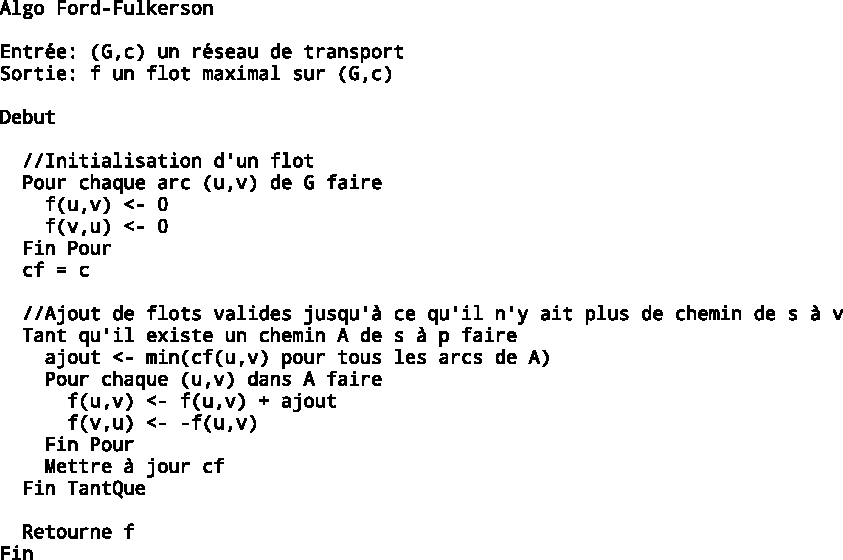
\includegraphics{Images/fig39.pdf}


\end{document}
